% CVPR 2024 Paper Template; see https://github.com/cvpr-org/author-kit

\documentclass[10pt,twocolumn,letterpaper]{article}

%%%%%%%%% PAPER TYPE  - PLEASE UPDATE FOR FINAL VERSION
% \usepackage[review]{Dycvpr}      % To produce the REVIEW version
% \usepackage{cvpr}              % To produce the CAMERA-READY version
\usepackage[pagenumbers]{cvpr} % To force page numbers, e.g. for an arXiv version

% Include other packages here, before hyperref.
\usepackage{graphicx}
\usepackage{amsmath}
\usepackage{amssymb}
\usepackage{booktabs}
\usepackage{algpseudocode}
\usepackage{algorithm}
\usepackage{mathtools}
\usepackage{stmaryrd}
\usepackage{trimclip}
\newcommand{\X}{\mathbf{X}} %
\newcommand{\Xset}{{\cal X}} %
\newcommand{\T}{\mathbf{T}} %
\newcommand{\Tset}{\mathcal{T}} %
\newcommand{\Tp}{\tilde{\mathbf{T}}} %
\newcommand{\Rp}{\tilde{\mathbf{R}}} %
\newcommand{\tp}{\tilde{\mathbf{t}}} %
\newcommand{\G}{\mathbf{G}} %
\newcommand{\Edge}{\mathcal{E}} %
\newcommand{\Gset}{\mathcal{G}} %
\newcommand{\g}{\mathbf{g}} %
\newcommand{\flow}{\mathbf{F}} %
\newcommand{\fpt}{\bm{f}} %
\newcommand{\Pm}{\mathbf{P}} %
\newcommand{\Pset}{\mathcal{P}} %
\newcommand{\Id}{\mathbf{I}} %
\newcommand{\R}{\mathbb{R}} %
\newcommand{\Rot}{\mathbf{R}} %
\newcommand{\tra}{\mathbf{t}} %
\newcommand{\Lap}{\mathbf{L}} %
\newcommand{\w}{\mathbf{w}} %
\newcommand{\Z}{\bm{\zeta}} %
\newcommand{\Zm}{\mathbf{Z}} %
\newcommand{\U}{\mathbf{U}} %
\newcommand{\segnet}{\varphi_{\mathrm{group}}} %
\newcommand{\flownet}{\varphi_{\mathrm{flow}}} %
\newcommand{\confnet}{\varphi_{\mathrm{conf}}} %
\newcommand{\Man}{\mathcal{M}} %
\newcommand{\one}{\mathbf{1}} %
\newcommand{\zero}{\mathbf{0}} %
\newcommand{\SOg}{\mathrm{SO}(3)} %
\newcommand{\Sm}{\mathbf{S}} %
\newcommand{\D}{\mathbf{D}} %
\newcommand{\gt}{\mathrm{gt}}   %
\newcommand{\wt}{\mathbf{w}}    %
\newcommand{\cf}{\textit{cf.}}    %
\newcommand{\wrt}{\text{w.r.t.}}
\newcommand{\etal}{\textit{et al.}}
% \newcommand{\refpaper}[1]{{\hypersetup{linkcolor={blue}}\ref{#1}}}


\newcommand{\mydots}{...}


\newcolumntype{Y}{>{\centering\arraybackslash}X}

\newtheorem{thm}{Theorem}
\newtheorem{remark}{Remark}
\newtheorem{cor}{Corollary}
\newtheorem{lemma}{Lemma}
\newtheorem{prop}{Proposition}
\newtheorem{dfn}{Definition}
\newtheorem{conj}{Conjecture}


\newcommand{\tmpeqno}{{\color{red} (TEMPEQ) }}

\newcommand{\jh}[1]{\textcolor[rgb]{0.0,0.0,1.0}{(Jiahui: #1)}}
\newcommand{\tolga}[1]{{\color{red} (Tolga: #1)} }

% \DeclareMathOperator{\sign}{sign}
\newcommand{\sign}{\operatorname{sign}}
\newcommand{\sas}{{\cal S} \alpha {\cal S} }

\crefname{section}{\S}{\S\S}
\crefname{subsection}{\S}{\S\S}

\newtheorem{assumption}{\textbf{H}\hspace{-3pt}}
\Crefname{assumption}{\textbf{H}\hspace{-3pt}}{\textbf{H}\hspace{-3pt}}
\crefname{assumption}{\textbf{H}}{\textbf{H}}

\newcommand{\insertimage}[4]{ %
\begin{figure}[t]
\centering
\includegraphics[scale=#1, clip=true]{figures/#2}
\caption{#3}
\label{#4}
\end{figure}
}

\newcommand{\insertimageC}[5]{ %
\begin{figure}[#5]
\centering
\includegraphics[width=#1\columnwidth, clip=true]{figures/#2}
\caption{#3}
\label{#4}
\end{figure}
}


\newcommand{\insertimageStar}[5]{ %
\begin{figure}[#5]
\centering
\includegraphics[width=#1\columnwidth, clip=true]{figures/#2}
\caption{#3}
\label{#4}
\end{figure}
}

\newcommand{\insertimageAsSubfig}[5]{ %
\begin{figure}[#5]
\begin{center}
\subfigbottomskip =-4in
\subfigure{
\includegraphics[width=#1\columnwidth]{figures/#2}
\label{#4}
}
\end{center}
\subfigbottomskip =-4in
\caption{#3}
\label{#4}
\end{figure}
}

\newcolumntype{d}[1]{D{.}{.}{#1}}
\newcolumntype{B}[3]{>{\boldmath\DC@{#1}{#2}{#3}}c<{\DC@end}}
% \DeclareMathOperator*{\argmax}{argmax}
\newcommand{\argmax}{\operatorname{argmax}}
% \DeclareMathOperator*{\argmin}{argmin}
\newcommand{\argmin}{\operatorname{argmin}}
\definecolor{tikz_gray}{RGB}{191,191,191}
\definecolor{tikz_lblue}{RGB}{93,138,210}
\definecolor{tikz_dblue}{RGB}{46,78,124}
\definecolor{tikz_lviolet}{RGB}{161,125,173}
\definecolor{tikz_dviolet}{RGB}{148,55,255}
\definecolor{tikz_rose}{RGB}{250,150,150}
\definecolor{tikz_pink}{RGB}{214,19,115}
\definecolor{tikz_lpink}{RGB}{255,138,216}

\newcommand{\overbar}[1]{\mkern 1.5mu\overline{\mkern-1.5mu#1\mkern-1.5mu}\mkern 1.5mu}

\DeclareRobustCommand{\legendsquare}[1]{%
  \tikz[baseline=(a.south)]{\node[#1, inner sep=.8ex, outer sep=0] (a) {};}%
}
\newcommand{\parahead}[1]{\noindent\textbf{#1}:\ }
\newcommand{\tabhead}[1]{\par\textbf{#1}}
\newenvironment{packed_itemize}
{\begin{itemize}
    \setlength{\itemsep}{1pt}
    \setlength{\parskip}{0pt}
    \setlength{\parsep}{0pt}
}{\end{itemize}}


\newcommand{\konrad}[1]{{\textcolor{blue}{\textbf{Konrad:} {#1}}}}
\newcommand{\andreas}[1]{{\textcolor{cyan}{\textbf{Andreas:} {#1}}}}
\newcommand{\zan}[1]{{\textcolor{brown}{\textbf{Zan:} {#1}}}}
\newcommand{\shengyu}[1]{{\textcolor{magenta}{\textbf{Shengyu:} {#1}}}}
\newcommand{\mikhail}[1]{{\textcolor{orange}{\textbf{Mikhail:} {#1}}}}
\newcommand{\cameraready}[1]{{\textcolor{blue}{{#1}}}}

\newcommand{\acro}{\textsc{Predator}}
\newcommand{\acroexplain}{\textbf{p}oint-cloud \textbf{re}gistration with \textbf{d}eep \textbf{at}tention to the \textbf{o}verlap \textbf{r}egion}





\sloppy
\definecolor{turquoise}{cmyk}{0.65,0,0.1,0.3}
\definecolor{purple}{rgb}{0.65,0,0.65}
\definecolor{dark_green}{rgb}{0, 0.5, 0}
\definecolor{orange}{rgb}{0.8, 0.6, 0.2}
\definecolor{red}{rgb}{0.8, 0.2, 0.2}
\definecolor{darkred}{rgb}{0.6, 0.1, 0.05}
\definecolor{blueish}{rgb}{0.0, 0.3, .6}
\definecolor{light_gray}{rgb}{0.7, 0.7, .7}
\definecolor{pink}{rgb}{1, 0, 1}
\definecolor{greyblue}{rgb}{0.25, 0.25, 1}


\newcommand{\CIRCLE}[1]{\raisebox{.5pt}{\footnotesize \textcircled{\raisebox{-.6pt}{#1}}}}

\newcommand{\expect}{\mathbb{E}}
\newcommand{\real}{\mathbb{R}}
\newcommand{\waymo}{\emph{Waymo}}
\newcommand{\nuscenes}{\emph{nuScenes}}

% \crefname{section}{\S}{\S\S}
% \crefname{subsection}{\S}{\S\S}
\crefname{section}{\text{Sec.}}{\text{Sec.}}
\crefname{subsection}{\text{Sec.}}{\text{Sec.}}
\crefname{equation}{\text{Eq}}{\text{Eq}}
\crefname{definition}{\text{Dfn.}}{\text{Dfn.}}
\crefname{tab}{\text{Tab.}}{\text{Tab.}}
\crefname{fig}{\text{Fig.}}{\text{Fig.}}
\crefname{table}{\text{Tab.}}{\text{Tab.}}
\crefname{figure}{\text{Fig.}}{\text{Fig.}}
\crefname{chapter}{\text{Chap.}}{\text{Chap.}}

\usepackage{blindtext}
\newcommand{\lorem}[1]{\todo{\blindtext[#1]}}

\renewcommand{\paragraph}[1]{\vspace{1em}\noindent\textbf{#1}.}


\newcommand{\lcircle}[1]{{\hspace{0.1em}\tikz\draw[#1,fill=#1] (0,0) circle (.4ex);}}

\makeatletter
\DeclareRobustCommand\onedot{\futurelet\@let@token\@onedot}
\def\@onedot{\ifx\@let@token.\else.\null\fi\xspace}

\def\eg{\emph{e.g}\onedot} \def\Eg{\emph{E.g}\onedot}
\def\ie{\emph{i.e}\onedot} \def\Ie{\emph{I.e}\onedot}
\def\cf{\emph{c.f}\onedot} \def\Cf{\emph{C.f}\onedot}
\def\etc{\emph{etc}\onedot} \def\vs{\emph{vs}\onedot}
\def\wrt{w.r.t\onedot} \def\dof{d.o.f\onedot}
\def\etal{\emph{et al}\onedot}
\makeatother

\newcommand{\ego}{\mathrm{ego}}
\newcommand{\pos}{\mathrm{pos}}
\newcommand{\geo}{\mathrm{ego}}     %
\newcommand{\pose}{\mathrm{pose}}
\newcommand{\obj}{\mathrm{obj}}
\newcommand{\trans}{\mathrm{trans}}
\newcommand{\type}{*}
\newcommand{\static}{\mathrm{static}}
\newcommand{\loss}{\mathcal{L}}
\newcommand{\Iset}{\mathcal{I}}
\newcommand{\tvec}{\mathbf{t}}
\newcommand{\Flow}{\mathbf{V}}
\newcommand{\s}{\mathbf{s}}
\newcommand{\x}{\mathbf{x}}
\newcommand{\quat}{\mathbf{q}}
\newcommand{\SEuc}{\mathrm{SE}(3)}
\newcommand{\Feature}{\mathbf{F}}
\newcommand{\feature}{\mathbf{f}}
\newcommand{\agfeature}{\tilde{\mathbf{f}}}
\newcommand{\pillar}{\mathbf{p}}
\newcommand{\point}{\mathbf{x}}
\newcommand{\offset}{\bm{\delta}}
\newcommand{\MLP}{\mathrm{MLP}}
\newcommand{\PN}{\mathrm{PN}}
\newcommand{\FG}{\mathrm{FG}}
\newcommand{\cat}{\mathrm{cat}}
\newcommand{\textoffset}{\mathrm{offset}}
\newcommand{\PC}{\mathbf{X}}
\newcommand{\PCset}{\mathcal{X}}
\newcommand{\bev}{\mathrm{base}}  %
\newcommand{\motion}{\mathrm{motion}}  %

\definecolor{lossred}{rgb}{1.0, 0.01, 0.24}
\definecolor{lossgreen}{rgb}{0.55, 0.71, 0.0}
\definecolor{lossblue}{rgb}{0.0, 0.44, 1.0}
\definecolor{lossyellow}{rgb}{1.0, 0.66, 0.07}
\definecolor{losspurple}{rgb}{0.76, 0.33, 0.76}
\definecolor{tab10orange}{rgb}{1.0, 0.7, 0.0}




\newcommand{\todo}[1]{{\textcolor{red}{\textbf{#1}}}}

\newcommand{\btau}{\boldsymbol{\tau}}
\newcommand{\bmu}{\boldsymbol{\mu}}
\newcommand{\beps}{\boldsymbol{\epsilon}}
\newcommand{\ba}{\mathbf{a}}
\newcommand{\bx}{\mathbf{x}}
\newcommand{\bc}{\mathbf{c}}

\newcommand{\map}{\boldsymbol{\mathcal{M}}}
\newcommand{\reals}{\mathbb{R}}
\newcommand{\normal}{\mathcal{N}}
\newcommand{\guide}{\mathcal{J}}


\newcommand{\name}{{{NeLF}}\xspace}

\definecolor{mygray}{RGB}{120, 120, 120}
\definecolor{myblue}{RGB}{68, 114, 196}
\definecolor{myorange}{RGB}{237, 125, 49}

\newcommand{\dir}{\mathbf{d}}
\newcommand{\origin}{\mathbf{o}}
\newcommand{\f}{\mathbf{f}}
\newcommand{\ray}{\mathbf{r}}
\newcommand{\density}{\sigma}
\newcommand{\opacity}{\alpha}
\newcommand{\reflectance}{\rho}
\newcommand{\radiance}{\mathbf{c}}
\newcommand{\intensity}{e}
\newcommand{\pdrop}{p_d}
\newcommand{\ptwo}{p_s}
\newcommand{\posfeat}{\mathbf{f}_{\text{pos}}}
\newcommand{\geofeat}{\mathbf{f}_{\text{geo}}}
\newcommand{\geofeatbar}{\bar{\mathbf{f}}_{\text{geo}}}
\newcommand{\dirfeat}{\mathbf{f}_{\text{dir}}}
\newcommand{\rangefeat}{\mathbf{f}_{\text{range}}}
\newcommand{\rayfeat}{\mathbf{f}_{\text{beam}}}
\definecolor{sem0}{rgb}{0.98431373, 0.70588235, 0.68235294}
\definecolor{sem1}{rgb}{0.70196078,0.80392157, 0.89019608}
\definecolor{sem2}{rgb}{0.8, 0.92156863, 0.77254902}
\definecolor{sem3}{rgb}{0.87058824, 0.79607843, 0.89411765}
\definecolor{ourgray}{rgb}{0.78, 0.78, 0.78}
\definecolor{error}{rgb}{0, 0.635, 1}
\definecolor{sdpoints}{rgb}{1.0, 0.706, 0.0}
\definecolor{hit}{rgb}{0.12156863,0.47058824,0.70588235}
\newcommand{\coolwarm}{\includegraphics[width=3em,height=0.8em]{main/images/coolwarm.png}}
\newcommand{\bwr}{\includegraphics[width=3em,height=0.8em]{main/images/bwr.png}}



\DeclarePairedDelimiter\parens{\lparen}{\rparen}
\DeclarePairedDelimiter\abs{\lvert}{\rvert}
\DeclarePairedDelimiter\norm{\lVert}{\rVert}
\DeclarePairedDelimiter\floor{\lfloor}{\rfloor}
\DeclarePairedDelimiter\ceil{\lceil}{\rceil}
\DeclarePairedDelimiter\braces{\lbrace}{\rbrace}
\DeclarePairedDelimiter\bracks{\lbrack}{\rbrack}
\DeclarePairedDelimiter\angles{\langle}{\rangle}

\crefname{section}{Sec.}{Secs.}
\Crefname{section}{Section}{Sections}
\Crefname{table}{Table}{Tables}
\crefname{table}{Tab.}{Tabs.}
\crefname{equation}{\text{Eq}}{\text{Eq}}
\crefname{equation}{Eq.}{Eq.}

\makeatletter
 \def\@textbottom{\vskip \z@ \@plus 1pt}
 \let\@texttop\relax
\makeatother


\newcommand{\dynfl}{DyNFL\xspace}
\newcommand{\rgb}{\mathbf{c}}
\newcommand{\pt}{\mathbf{p}}
\newcommand{\feat}{\gamma}
\newcommand{\tnt}{Tanks and Temples\xspace}
\newcommand{\deriv}[2]{\frac{\partial #1}{\partial #2}}
\newcommand{\sdf}{f}
\newcommand{\curv}{\frac{1}{2} \nabla^2 \sdf(\pos)}
\newcommand{\dist}{\mathbf{d_{f}}}
\newcommand{\leik}{\mathcal{L}_{\text{eik}}}
\newcommand{\transmittance}{\mathcal{T}}
\newcommand{\bwrDyNFL}{\includegraphics[width=3em,height=0.8em]{Figures/bwr.png}}
\newcommand{\exponential}[1]{\text{exp}\left(#1\right)}
\newcommand{\rayfeatideal}{\mathbf{f}_{\text{ray}}}
\newcommand{\reflectivity}{\rho}
\newcommand{\weight}{\alpha}
\newcommand{\rayOri}{\mathbf{o}}
\newcommand{\rayDir}{\mathbf{d}}
% \usepackage{natbib}
% \bibliographystyle{abbrvnat}
% \setcitestyle{authoryear,open={((},close={))}} %Citation-related commands

\makeatletter
\DeclareRobustCommand{\shortto}{%
  \mathrel{\mathpalette\short@to\relax}%
}

\newcommand{\short@to}[2]{%
  \mkern2mu
  \clipbox{{.5\width} 0 0 0}{$\m@th#1\vphantom{+}{\shortrightarrow}$}%
  }
\makeatother
\newcommand{\xing}[1]{{\textcolor{blue}{\textbf{Xing: {#1}}}}}
\newcommand{\shengyu}[1]{{\textcolor{red}{\textbf{Shengyu:} {#1}}}}
\newcommand{\orl}[1]{{\textcolor{orange}{\textbf{OrL:} {#1}}}}
\newcommand{\stefan}[1]{{\textcolor{pink}{\textbf{Stefan:} {#1}}}}
\newcommand{\hanfeng}[1]{{\textcolor{green}{\textbf{Hanfeng:} {#1}}}}
\newcommand{\dynfl}{DyNFL\xspace}
\newcommand{\dynfl}{DyNFL\xspace}
\newcommand{\rgb}{\mathbf{c}}
\newcommand{\pos}{\mathbf{p}}
\newcommand{\feat}{\gamma}
\newcommand{\tnt}{Tanks and Temples\xspace}
\newcommand{\deriv}[2]{\frac{\partial #1}{\partial #2}}
\newcommand{\sdf}{f}
\newcommand{\normal}{\nabla \sdf(\pos)}
\newcommand{\curv}{\frac{1}{2} \nabla^2 \sdf(\pos)}
\newcommand{\x}{\mathbf{x}}
\newcommand{\dir}{\mathbf{d}}
\newcommand{\origin}{\mathbf{o}}
\newcommand{\dist}{\mathbf{d_{f}}}
\newcommand{\f}{\mathbf{f}}
\newcommand{\real}{\mathbb{R}}
\newcommand{\ray}{\mathbf{r}}
\newcommand{\density}{\sigma}
\newcommand{\opacity}{\alpha}
\newcommand{\reflectance}{\rho}
\newcommand{\radiance}{\mathbf{c}}
\newcommand{\intensity}{e}
\newcommand{\pdrop}{p_d}
\newcommand{\ptwo}{p_s}
\DeclareMathOperator*{\argmax}{arg\,max}
\DeclareMathOperator*{\argmin}{arg\,min}
\newcommand{\leik}{\mathcal{L}_{\text{eik}}}
\newcommand{\trans}{\mathcal{T}}
\newcommand{\bwrDyNFL}{\includegraphics[width=3em,height=0.8em]{Figures/bwr.png}}
\newcommand{\exponential}[1]{\text{exp}\left(#1\right)}

\newcommand{\posfeat}{\mathbf{f}_{\text{pos}}}
\newcommand{\geofeat}{\mathbf{f}_{\text{geo}}}
\newcommand{\geofeatbar}{\bar{\mathbf{f}}_{\text{geo}}}
\newcommand{\dirfeat}{\mathbf{f}_{\text{dir}}}
\newcommand{\rangefeat}{\mathbf{f}_{\text{range}}}
\newcommand{\rayfeat}{\mathbf{f}_{\text{ray}}}
\newcommand{\cat}{\mathrm{cat}}
\newcommand{\reflectivity}{\rho}
\newcommand{\weight}{\alpha}
\newcommand{\rayOri}{\mathbf{o}}
\newcommand{\rayDir}{\mathbf{d}}
% It is strongly recommended to use hyperref, especially for the review version.
% hyperref with option pagebackref eases the reviewers' job.
% Please disable hyperref *only* if you encounter grave issues, e.g. with the
% file validation for the camera-ready version.
%
% If you comment hyperref and then uncomment it, you should delete
% ReviewTempalte.aux before re-running LaTeX.
% (Or just hit 'q' on the first LaTeX run, let it finish, and you
%  should be clear).
% \usepackage[pagebackref,breaklinks,colorlinks]{hyperref}
\definecolor{cvprblue}{rgb}{0.21,0.49,0.74}
\usepackage[pagebackref,breaklinks,colorlinks,citecolor=cvprblue]{hyperref}


% Support for easy cross-referencing
\usepackage[capitalize]{cleveref}
\crefname{section}{Sec.}{Secs.}
\Crefname{section}{Section}{Sections}
\Crefname{table}{Table}{Tables}
\crefname{table}{Tab.}{Tabs.}




%%%%%%%%% PAPER ID  - PLEASE UPDATE
\def\paperID{2088} % *** Enter the CVPR Paper ID here
\def\confName{CVPR}
\def\confYear{2024}




\title{Supplementary material: Dynamic LiDAR Re-simulation using Compositional Neural Fields}

\setcounter{section}{0}
\renewcommand\thesection{\Alph{section}}
\newcommand{\manuallabel}[2]{\def\@currentlabel{#2}\label{#1}}
\makeatother
\newcommand{\refpaper}[1]{{\hypersetup{linkcolor={red}}\ref{#1}}}
\allowdisplaybreaks
\begin{document}
\maketitle




In this supplementary material, we first provide additional information about the datasets for our evaluations and implementation details of our proposed method in~\cref{sec:sup_dataset}. Next, we present more qualitative results in~\cref{sec:sup_visual}. Please also check the supplemental video for more results showcasing our performance. Finally, we provide the complete derivations of the SDF-based volume rendering for active sensor in~\cref{sec:sup_sdf_vol_render}. 

\subsection{Datasets and implementation details}\label{sec:sup_dataset}
\paragraph{\textit{Waymo Dynamic}} For the \textit{Waymo Dynamic} dataset, we take them from 4 scenes of \textit{Waymo Open Dataset}~\cite{sun2020scalability}. There are multiple moving vehicles inside each scene. 50 consecutive frames are taken from each scene for our evaluation. The vehicles are deemed as \textit{dynamic} if the speed is $>1\,$m/s. in any of the 50 frames. The corresponding scene IDs on \textit{Waymo Open Dataset} for our selected scenes are shown as follows:
\begin{table}[t]
    \setlength{\tabcolsep}{4pt}
    \renewcommand{\arraystretch}{1.2}
	\centering
	\resizebox{0.6\columnwidth}{!}{
    \begin{tabular}{l|c}
    \toprule
    & Scene ID \\
    \midrule
    Scene 1 & 1083056852838271990\_4080\_000\_4100\_000 \\
    Scene 2 & 13271285919570645382\_5320\_000\_5340\_000 \\
    Scene 3 & 10072140764565668044\_4060\_000\_4080\_000 \\
    Scene 4 & 10500357041547037089\_1474\_800\_1494\_800 \\
    \bottomrule
    \end{tabular}
    }
\end{table}

\paragraph{Ours} 
Our model is implemented based on nerfstudio\cite{nerfstudio}. For the static neural field, we sample $N_s=512$ points in total, with $N_u=256$ uniformly sampled points and $N_i=256$ weighted sampled points with 8 upsample steps. In each upsample step, 32 points are sampled based on the weight distribution of the previously sampled points. For each dynamic neural field, we sample $N_s=128$ points in total, with $N_u=64$ uniformly sampled points and $N_i=64$ weighted sampled points with 4 upsample steps. During training, we minimize the loss function using the Adam~\cite{kingma2014adam} optimiser, with an initial learning rate of 0.005. It linearly decays to 0.0005 towards the end of training. For the loss weights, we use $w_{\zeta}=3, w_{e}=50, w_{\text{drop}}=0.15, w_{s}=1$, and  $w_{\text{eik}}=0.3$. The batch size is 4096 and we train the model for 60000 iterations on a single RTX3090 GPU with float32 precision.

\paragraph{LiDARsim} We re-implement the LiDARsim~\cite{manivasagam2020lidarsim} as one of our baselines. 
First, we estimated point-wise normal vectors by considering all points within a 20 cm radius ball within the training set. Following this, we applied voxel down-sampling~\cite{tang2022torchsparse}, employing a 4 cm voxel size to reconstruct individual disk surfels at each point. The surfel orientation is defined based on the estimated normal vector. During inference, we apply the ray-surfel intersections test to determine the intersection points, thus the range and intensity values. We select a fixed surfel radius of 6 cm for the \textit{Waymo} dataset and 12 cm for the \textit{Town} dataset.
To handle dynamic vehicles, we follow LiDARsim~\cite{manivasagam2020lidarsim} by aggregating the LiDAR points for each vehicle from all the training frames and representing them in the \textit{canonical} frame of each vehicle. During inference, we transform all the aggregated vehicle points from their \textit{canonical} frames to the world frame and run ray-surfel intersection.

\paragraph{UniSim} 
We re-implement UniSim's~\cite{yang2023unisim} rendering process for LiDAR measurements by replacing our ray-drop test-based neural fields composition method with its joint rendering method. For every ray $\mathbf{r} (\mathbf{o},\mathbf{d})$, we begin by conducting an intersection test with all dynamic bounding boxes in the scene to identify the near and far limits. We then uniformly sample 512 points along each ray, assigning each point to either a dynamic neural field, if it falls within a dynamic bounding box, or to the static neural field otherwise. After sampling, we query the SDF and intensity values from the relevant neural fields. Finally, using the SDF-based volume rendering formula in Eq.~\ref{eq:depth_render} for active sensors, we calculate the weights and perform the rendering. Note that we use the same neural field architecture as in our method.
\begin{figure*}[t!]
  \centering
   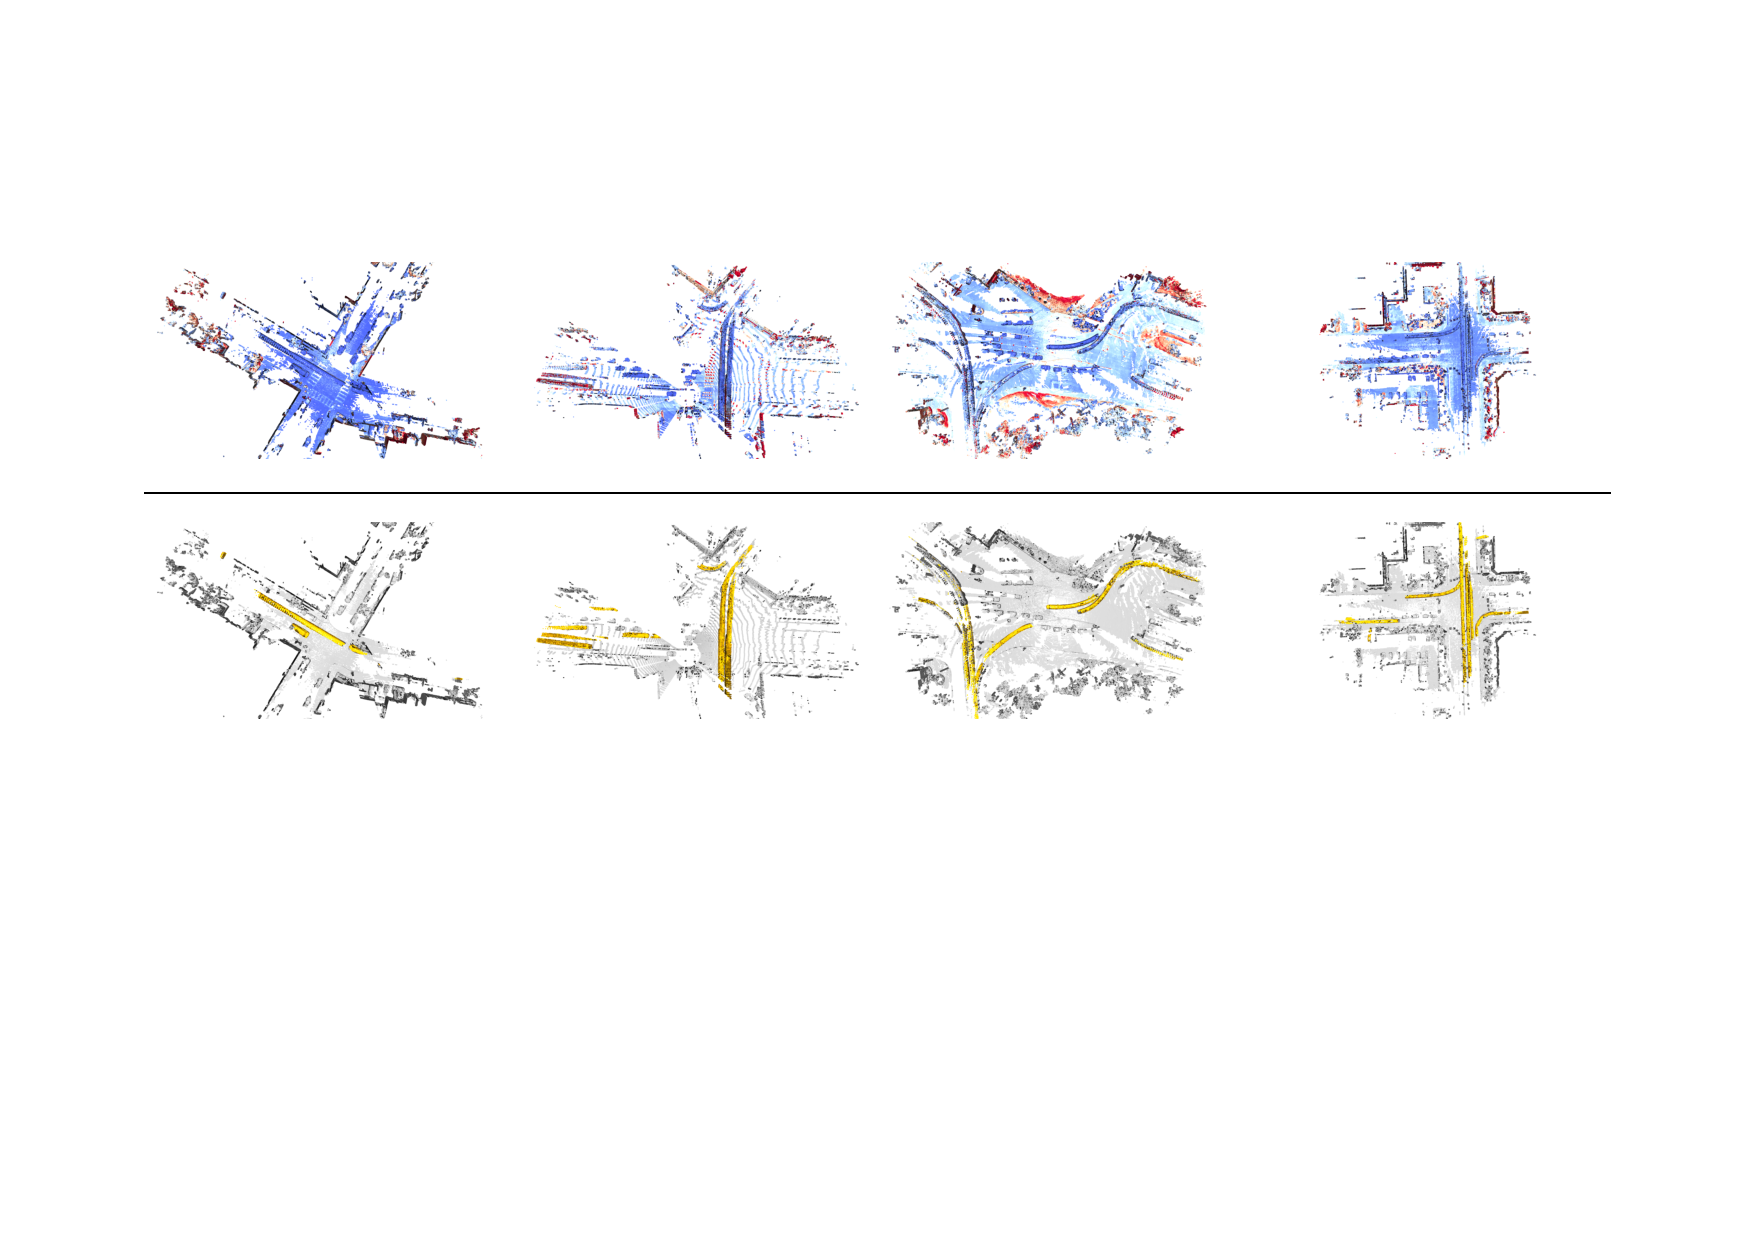
\includegraphics[width=1\columnwidth]{Figures_sup/4_scenes_sup.pdf}
   \caption{Visualization of 4 selected scenes from \textit{Waymo Dynamic} dataset. For each scene, we aggregate 50 frames. In the first row, points are color-coded by the intensity values(0 ~\bwrDyNFL~ 0.25). In the second row, dynamic vehicles are painted as \textcolor{yellow}{yellow}.}
   \label{fig:4_scenes_supp}
\end{figure*}

\begin{figure*}[t!]
  \centering
   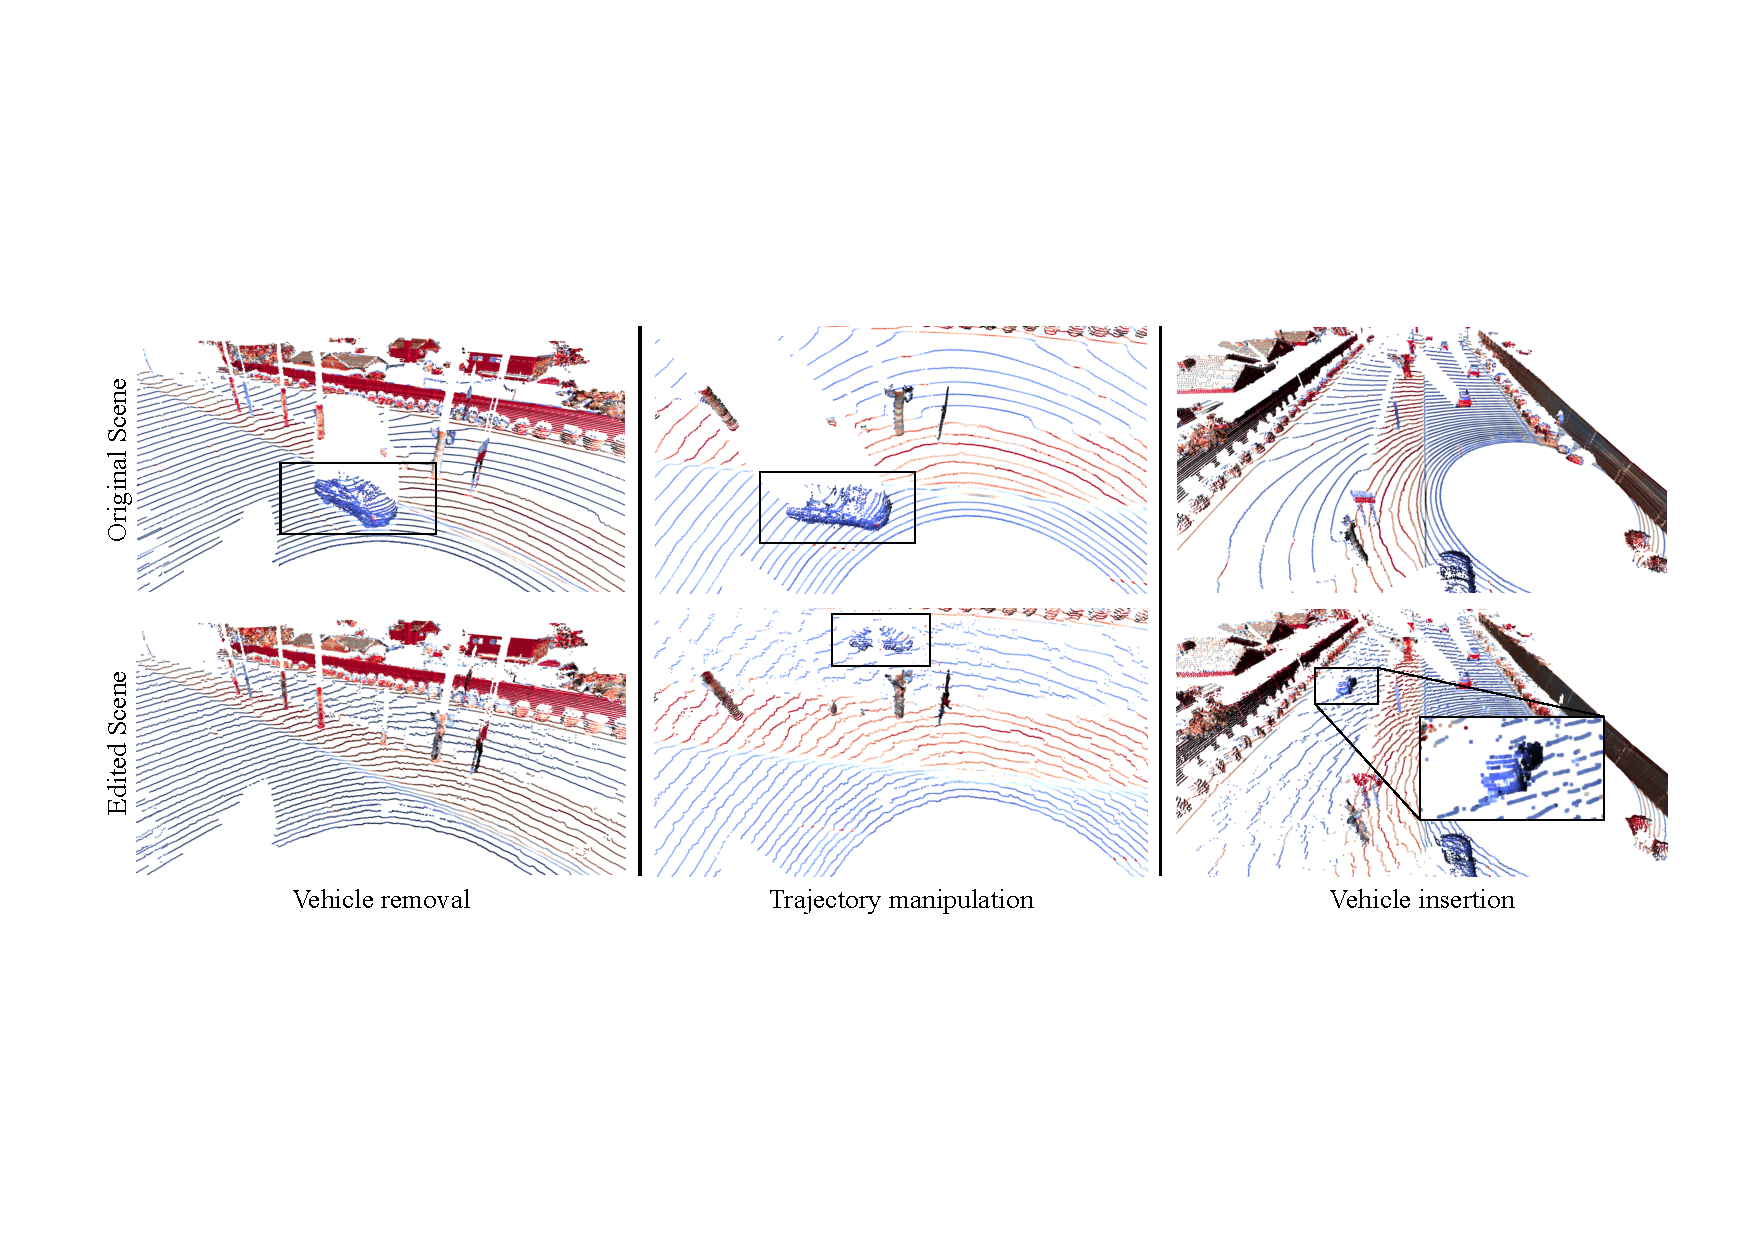
\includegraphics[width=1\columnwidth]{Figures_sup/supp_scene_edit.pdf}
   \caption{Visualization of scene editing capabilities. We showcase 3 kinds of scene editing capabilities including vehicle removal(left), trajectory manipulation(middle) and vehicle insertion(right). The first row represents the original scenes, the second row demonstrates the scenes after editing. All points are color-coded by the intensity values(0 ~\bwrDyNFL~ 0.25).}
   \label{fig:scene_editing_supp}
\end{figure*}

\section{More qualitative results}\label{sec:sup_visual}
In this section, we provide more qualitative results. In \cref{fig:4_scenes_supp}, we showcase the 4 scenes from \textit{Waymo dynamic} dataset. We show additional scene editing results in~\cref{fig:scene_editing_supp}. Please check the supplementary videos for more qualitative results.


\section{SDF-based volume rendering for active sensor}\label{sec:sup_sdf_vol_render}
In this section, we start by introducing the preliminary of NeRF~\cite{mildenhall2020nerf} following terminology as described in~\cite{tagliasacchi2022volume}. Then we provide the full derivation of the SDF-based volume rendering for active sensor. 

\subsection{Preliminary}\label{sec:supp_pre}
\paragraph{Density}
For a ray emitted from the origin $\origin \in \real^3$ towards direction $\dir \in \real^3$, the \textit{density} $\density_\zeta$ at range $\zeta$ indicates the likelihood of light interacting with particles at that point $\ray_\zeta = \origin + \zeta \dir$. This interaction can include absorption or scattering of light. In passive sensing, density $\density$ is a critical factor in determining how much light from the scene's illumination is likely to reach the sensor after passing through the medium.
\paragraph{Transmittance} quantifies the likelihood of light traveling through a given portion of the medium without being scattered or absorbed. Density is closely tied to the transmittance function $\trans(\zeta)$, which indicates the probability of a ray traveling over the interval $[0, \zeta)$ without hitting any particles. Then the probability $\trans(\zeta {+} d\zeta)$ of \emph{not} hitting a particle when taking a differential step $d\zeta$ is equal to $\trans(\zeta)$, the likelihood of the ray reaching $\zeta$, times $(1 - d\zeta \cdot \density(\zeta))$, the probability of not hitting anything during the step:
% 
\begin{align}
\trans(\zeta+d\zeta) =& \trans(\zeta) \cdot (1 - d\zeta \cdot \density(\zeta))
\\
\frac{\trans(\zeta+d\zeta) - \trans(\zeta)}{d\zeta} \equiv& \trans'(\zeta) = -\trans(\zeta) \cdot \sigma(\zeta) 
\label{eq:derivative}
\end{align}
% 
We solve the differential equation as follows:
%
\begin{align}
\trans'(\zeta) &= -\trans(\zeta) \cdot \density(\zeta) \\
\frac{\trans'(\zeta)}{\trans(\zeta)} &= -\density(\zeta) \\
\int_a^b \frac{\trans'(\zeta)}{\trans(\zeta)} \; d\zeta &= -\int_a^b \density(\zeta) \; d\zeta \\
\left. \log \trans(\zeta) \right|_a^b &= -\int_a^b \density(\zeta) \; d\zeta \\
\trans(a \rightarrow b) \equiv \frac{\trans(b)}{\trans(a)} &= \exponential{-\int_a^b \density(\zeta) \; d\zeta}   
\end{align}
% 
Hence, for a ray segment between $\zeta_0$ and $\zeta$, transmittance is given by:

\begin{equation}
\trans_{\zeta_0 \rightarrow \zeta} \equiv \frac{\trans_{\zeta}}{\trans_{\zeta_0}} = exp({-\int_{\zeta_0}^\zeta \density_t dt})\;,
\label{eq:trans_ab}
\end{equation}
which leads to following factorization of the transmittance:
\begin{equation}
\trans_{\zeta} = \trans_{0 \rightarrow \zeta_0} \cdot \trans_{\zeta_0 \rightarrow \zeta}\;.
\label{eq:factor}
\end{equation}

\paragraph{Opacity}Opacity is the complement of transmittance and represents the fraction of light that is either absorbed or scattered in the medium. In a homogeneous medium with constant density $\density$  the opacity for a segment $[\zeta_j, \zeta_{j+1}]$ of length $\Delta \zeta$ is given by $\opacity_{\zeta_j} = 1 - exp(-\density \cdot \Delta \zeta)$
\subsection{SDF-based volume rendering for active sensor}\label{sec:sdf_active}
NeuS\cite{wang2021neus} derives the opaque density based on the SDF which is:
\begin{equation}
\begin{split}
\density_{\zeta_i} =&  \max\left(\frac{-\frac{d\Phi_s}{d\zeta_i}(f(\zeta_i))}{\Phi_s(f(\zeta_i))},0\right)\\
                  =& \max\left(\frac{-(\nabla f(\zeta_i)\cdot \mathbf{v})\phi_s(f(\zeta_i))}{\Phi_s(f(\zeta_i))}, 0\right)
\end{split}
\label{eq:sigmoid_density_}
\end{equation}
where $\Phi_s$ represents the Sigmoid function, $f$ is the SDF function that maps a range $\zeta$ to the SDF value of the point position $\origin + \dir * \zeta$. Note that the integral term is computed by
\begin{equation}
\int \frac{-(\nabla f(\zeta)\cdot \mathbf{v})\phi_s(f(\zeta))}{\Phi_s(f(\zeta))}d\zeta = -\ln(\Phi_s(f(\zeta))) + C,
\label{eq:intergration_density}
\end{equation}
We extend the density-based volume rendering for active sensor to SDF-based. Starting from the passive SDF-based volume rendering \cite{wang2021neus}, We substitute the density $\tilde{\density}$ with opaque density in \ref{eq:sigmoid_density_}
and evaluate the radiant power integrated from ray segment [a,b] with constant reflectivity $\reflectivity_a$.

Consider the case where $-(\nabla f(\zeta)\cdot \mathbf{v})>0$ within the ray segment $[a,b]$, we have
\begin{align}
P(a \rightarrow b)
&= \int_a^b \trans^2(a\rightarrow t) \cdot \tilde{\density}_t \cdot \reflectivity(t)  \; dt
\\
&= \reflectivity_a \int_a^b \trans^2(a\rightarrow t) \cdot \tilde{\density}_t \; dt
\\
&= \reflectivity_a \int_a^b \exponential{-\int_a^t 2\tilde{\density}(u) \; du} \cdot \tilde{\density}_t \; dt
\\
&= \reflectivity_a \int_a^b \exponential{-2\int_a^t \tilde{\density}(u) \; du} \cdot \tilde{\density}_t \; dt
\\
&= \reflectivity_a \int_a^b \exponential{\left. 2\ln(\Phi_s(f(u)))\right|_a^t} \cdot \tilde{\density}_t \; dt
\\
&= \reflectivity_a \int_a^b \exponential{2\ln(\Omega_t) - 2\ln(\Omega_a)} \cdot \tilde{\density}_t \; dt 
\\
&= \reflectivity_a \int_a^b \frac{{\Omega_t}^2}{{\Omega_a}^2} \cdot \tilde{\density}_t \; dt ~~~~\text{\textbf{let} $\Omega_x = \Phi_s(f(x))$}
\\
&= \frac{\reflectivity_a}{{\Omega_a}^2} \int_a^b {\Omega_t}^2 \cdot \tilde{\density}_t \; dt 
\\
&= \frac{\reflectivity_a}{{\Omega_a}^2} \int_a^b -\frac{d\Phi_s}{dt}(f(t)) \cdot \Phi_s(f(t)) \; dt 
\\
&= \frac{\reflectivity_a}{{\Omega_a}^2} ( \left. -\frac{1}{2}{\Phi_s(f(t))}^2 \right|_a^b) \\
&= \frac{\reflectivity_a}{{\Omega_a}^2} (\frac{1}{2}{\Phi_s(f(a))}^2 -\frac{1}{2}{\Phi_s(f(b))}^2 )\\
&= \frac{{\Phi_s(f(a))}^2 -{\Phi_s(f(b))}^2}{{2\Phi_s(f(a))}^2} \cdot \reflectivity_a 
\label{eq:homogeneous}
\end{align}

Consider the case where $-(\nabla f(\zeta)\cdot \mathbf{v})<0$ within the ray segment $[a,b]$, we have
\begin{align}
P(a \rightarrow b)
&= \int_a^b \trans^2(a\rightarrow t) \cdot \tilde{\density}_t \cdot \reflectivity(t)  \; dt
\\
&= \int_a^b \trans^2(a\rightarrow t) \cdot 0 \cdot \reflectivity(t)  \; dt
\\
&= 0
\end{align}
Hence we conclude 
\begin{align}
P(a \rightarrow b)
&= \max\left(\frac{{\Phi_s(f(a))}^2 -{\Phi_s(f(b))}^2}{{2\Phi_s(f(a))}^2},0\right) \cdot \reflectivity_a 
\end{align}

\paragraph{Volume rendering of piecewise constant data}
Combining the above, we can evaluate the volume rendering integral through a medium with piecewise constant reflectivity:
% 
\begin{align}
P(\zeta_{N+1}) &= \sum_{n=1}^N \int_{\zeta_n}^{\zeta_{n+1}} \trans^2(\zeta) \cdot \tilde{\density}_{\zeta} \cdot \reflectivity_{\zeta_n} \; d\zeta
\\
&= \sum_{n=1}^N \int_{\zeta_n}^{\zeta_{n+1}} \trans^2_{\zeta_n} \cdot \trans^2(\zeta_n \shortto \zeta) \cdot \tilde{\density}_{\zeta} \cdot \reflectivity_{\zeta_n} \; d\zeta 
\\
&= \sum_{n=1}^N \trans^2_{\zeta_n}  \int_{\zeta_n}^{\zeta_{n+1}} \trans^2(\zeta_n \rightarrow \zeta) \cdot \tilde{\density}_{\zeta} \cdot \reflectivity_{\zeta_n} \; d\zeta \\
&=\sum_{n=1}^N \trans^2_{\zeta_n} P(\zeta_n \rightarrow \zeta_{n+1})
\\
&= \sum_{n=1}^N \trans^2_{\zeta_n} \cdot \tilde{\weight}_{\zeta_n} \cdot \reflectivity_{\zeta_n},
\end{align}

where 
\begin{align}
\tilde{\weight}_{\zeta_n} \equiv \max\left(\frac{{\Phi_s(f(\zeta_n)}^2 -{\Phi_s(f(\zeta_{n+1}))}^2}{{2\Phi_s(f(\zeta_n))}^2},0\right)
\end{align}

The discrete accumulated transmittance $\trans$ can be calculated as follows:

Consider the case where $-(\nabla f(\zeta)\cdot \mathbf{v}) > 0$ in $[\zeta_n, \zeta_{n+1}]$: 
%
\begin{align}
\trans_{\zeta_n} 
&=\prod_{i=1}^{n-1}(\exp(-\int_{\zeta_n}^{\zeta_{n+1}}\tilde{\density}_\zeta \; d\zeta) \\
&= \prod_{i=1}^{n-1}(\frac{\Phi_s(f(\zeta_{n+1}))}{\Phi_s(f(\zeta_n))})\\
\trans^2_{\zeta_n}
&= \prod_{i=1}^{n-1}(\frac{{\Phi_s(f(\zeta_{n+1}))}^2}{{\Phi_s(f(\zeta_n))}^2})\\
&= \prod_{i=1}^{n-1}(1-2\tilde{\weight}_{\zeta_n})
\label{eq:dicrete_transmittance}
\end{align}

Consider the case where $-(\nabla f(\zeta)\cdot \mathbf{v}) < 0$ in $[\zeta_n, \zeta_{n+1}]$: 
\begin{align}
\trans_{\zeta_n} 
&=\prod_{i=1}^{n-1}(\exp(-\int_{\zeta_n}^{\zeta_{n+1}}\tilde{\density}_\zeta \; d\zeta) = \prod_{i=1}^{n-1}(1)
\\
\trans^2_{\zeta_n} &= \prod_{i=1}^{n-1}(1^2) = \prod_{i=1}^{n-1}(1-2\tilde{\weight}_{\zeta_n})
\end{align}
In conclusion, the radiant power can be reformulated as:

\begin{align}
P(\zeta_{N+1}) = \sum_{n=1}^N \trans^2_{\zeta_n} \cdot \tilde{\weight}_{\zeta_n} \cdot \reflectivity_{\zeta_n}
\label{eq:final_radiant2}
\end{align}
where $\trans^2_{\zeta_n} = \prod_{i=1}^{n-1}(1-2\tilde{\weight}_{\zeta_i})$


\paragraph{Depth volume rendering of piecewise constant data}

Note that $\tilde{\weight}_{\zeta_n} \in [0, 0.5], \trans^2_{\zeta_n} \in [0,1], \sum_{n=1}^N \trans^2_{\zeta_n} \cdot \tilde{\weight}_{\zeta_n} = 0.5$, for depth volumetric rendering, we have 
\begin{align}
    \zeta = \sum_{n=1}^N 2 \cdot \trans^2_{\zeta_n} \cdot \tilde{\weight}_{\zeta_n} \cdot \zeta_n
    =\sum_{n=1}^N w_n \cdot \zeta_n
    \label{eq:depth_render}
\end{align}
where $w_n = 2\tilde{\weight}_{\zeta_n} \cdot \prod_{i=1}^{n-1}(1-2\tilde{\weight}_{\zeta_i})$
% 
\begin{table}[t]
\setlength{\tabcolsep}{4pt}
\renewcommand{\arraystretch}{1.2}
\centering
\resizebox{0.99\columnwidth}{!}{
\begin{tabular}{l|ccc|ccc}
\toprule
& \multicolumn{3}{c|}{Vehicle} & \multicolumn{3}{c}{Background} \\
Method & Recall $\uparrow$ & Precision $\uparrow$ & IoU $\uparrow$ & Recall $\uparrow$ & Precision $\uparrow$ & IoU $\uparrow$ \\
\midrule
i-NGP~\cite{mueller2022instant} & \underline{94.8} & 89.7 & \underline{85.6} & 98.7 & \underline{99.4} & \underline{98.1}\\
DS-NeRF~\cite{deng2021depth} & 91.4 & 88.9 & 82.2 & 98.7 & 99.1 & 97.8\\
URF~\cite{rematas2021urban} & 93.8 & 89.0 & 84.1 & 98.6 & 99.3 & 97.9\\
Lidarsim~\cite{manivasagam2020lidarsim} & 92.2 & 74.4 & 70.2 & 95.9 & 99.1 & 95.1\\
NFL~\cite{Huang2023nfl} & \textbf{95.7} & \underline{91.2} & \textbf{87.6} & \underline{98.8} & \textbf{99.5} & \textbf{98.3}\\
Ours & 91.4 & 89.2 & 82.3 & \underline{98.8} & 98.9 & 97.7\\
\bottomrule
\end{tabular}
}
\caption{Semantic segmentation results on \textit{Waymo Interp.} dataset.}
\label{tab:supp_sem_seg_interp}
\end{table}

%%%%%%%%% REFERENCES
{\small
\bibliographystyle{ieeenat_fullname}
\bibliography{main}
}

\end{document}
